
%\section{UI Gesture Collection}
%
%In order to create a mapping from commands, as issued by the users, to a set of individual robot programs for multi-robot command and control, the gesture set for the commands must first be specified. 
%Multitouch gesture sets as a command language for controlling robots have been developed by an empirical process with naive users \citep{Micire:2009:ANG:1731903.1731912}. 
%These gestures frequently consisted of sequences of gestures that roughly fit the linguistic structure of a sentence, with the first gesture indicating the subject of the sentence, and the next gesture indicating a verb and possibly an object. 
%As a consequence, the gestures form a sort of language, and commands are sentences in the gesture language.
%A user might select a group of robots by circling them. 
%These robots would be the subject of the ``sentence''.
%Then the user might draw a path or tap a spot on a map, indicating that the robots should ``go here''. 
%Taken all together, the sentence could be read as ``these robots, follow this line to this location'', with the referents disambiguated by the locations of the command gesture on the screen.
%
%One way to define such an interface would be to select a fixed set of gestures, and then train the users to use those gestures when they interact with the system. 
%However, if the system is not one that the users use frequently, they will forget the training. 
%Since the advent of multitouch interfaces for smartphones and the trackpads of some laptops, many users already have some prior experience with multitouch gesture controls in everyday life. 
%Multitouch gestures can also be imitations of the way the users would expect to interact with material objects. 
%For example, zooming out of a map view by pinching two fingers together imitates the distant points of the map becoming closer together, indicating outward zoom, and spreading the fingers imitates stretching a smaller region to cover the screen for an inward zoom. 
%From these ``naturalistic'' expectations and daily use, users already have some idea of how a multitouch user interface can work. 
%If the interface fulfills the users' expectations, the users will find it easier to learn to use. 
%
%In other work, for each available command, one or two gestures were sufficient to cover the gestures used by 60\% or more of the users\citep{Micire:2009:ANG:1731903.1731912}. 
%However, it  is possible that there is no common gesture across users for a given task.
%If no two users use the same gesture for the same commands, or, more generally, there is very poor inter-user similarity for the gestures chosen to issue a command, then the approach of defining gestures from the user input does not offer useful guidance. 
%
%In order to determine if the chosen gestures change with the size of the swarm, tests will be conducted with varying swarm sizes performing the same tasks. 
%The swarm used for these tests will be large, with the lower bound on its size being significantly larger than the number of fingers a user could potentially gesture with. 
%In order to have a less tongue-in-cheek definition of ``large'', the scale required for a swarm to be considered ``large'' will be determined empirically.
%It is expected that there exists a transition point for the number of members in a swarm where users will stop interacting with the UI representation of the members of the swarm as individuals, and attempt to interact with the representations as groups or collections. 
%
%A large swarm is, then, a swarm with a number of members above the point at which such a transition occurs

\subsection{Introduction}

Multitouch gestural interfaces, like those found on tablets and smartphones, offer the possibility of a very direct user experience, especially compared to the Windows, Icons, Mouse, Pointer (WIMP) interface design. 
Rather than, for example, using an arrow key to scroll in a document, the user can drag the document directly, as though they were sliding a long piece of paper on a table. 

This directness is a hallmark of what has come to be called Natural User Interfaces, or NUI. 
A natural user interface is one that allows the user to re-use existing skills and natural motions to interact directly with content \citep{blakeNUIWin}. 
In practice, this means that the elements of the interaction are actions such as pointing and other gestures, drawing with a pen, speech, gaze, and so forth, rather than computer-specific interface devices. 
By way of contrast, the command line interface is defined in terms of typing with some form of keyboard, and the graphic user interface is (in most cases), defined in terms of mouse actions. 

However, as the number of operations the user wishes to perform increases, the limitations of multitouch screens become more apparent. 
Screens are flat, and so only afford 2-dimensional gestures, such as dragging, poking, and tapping. 
Even if the screen depicts a 2-dimensional projection of a 3-dimensional world, operations that would make sense in the 3D world, such as grasping, have to be mapped to the 2-dimensional space of operations to be performed. 
Typically, the gestures that the user uses to perform the available operations are chosen by the interface developer, and the user is trained to perform them, possibly by a short tutorial program \citep{wobbrock2009user, vanacken2008ghosts, freeman2009shadowguides}. 

Unfortunately, the use of screens with interactions inspired by the affordances of physical objects leads to the user having to decide between ``natural'' skills and motions, which are used on physical objects, and the skills and actions used with screens: single-point dragging and clicking. 
Most users understand that they are looking at pictures of things on a screen, and so default to single-point interactions \citep{vanacken2008ghosts}.

However, the behavior of users interacting with an NUI device is not solely informed by their intuitions about the physical objects represented on the screen. 
Smartphones, tablets, and other multitouch user interface devices, as well as specific types of computer programs, such as CAD and realtime strategy game programs, also inform the user's expectations about interactions with new interfaces. 
Rather than claiming that the users are untrained, and the gestures are ``intuitive'', it would be more accurate to claim that the users already have a form of training, from the devices that they use in their daily lives. 
We attempt to discover the gestures that users would choose themselves, based on their own thinking about the interface and their own past experience with computer technology such as tablets, smartphones, and video games. 

This work is an extension of previous work that used a similar process to discover user interface gestures for single or small groups of robots \citep{Micire:2009:ANG:1731903.1731912}. We extend this method from groups to larger swarms of robots, in an attempt to discover if the gestures that users select vary with the number of robots available.

More specifically, it is hypothesized that there exists a swarm size beyond which users will transition from treating the swarm robots as individuals to interacting with the robots in small groups or as a single large group. 
This transition point will be apparent because of a change in the gesture set that users choose to interact with the swarm. 
Rather than issuing one command for each robot, the user will instead use commands that control the bulk of the robots as a cloud or flock, but may leave some robots unused. 
For example, the user may switch from selecting robots as individuals to shaping the group as if sculpting, with pushing and pinching to ``carry'' groups around. 
The user may also change how they indicate which robots are to be interacted with. 
Rather than selecting each robot by clicking on it, the user might circle a group they want to use, or simply assume that the same command is issued to all robots by default. 
The size of the swarm where changes in the user gestures occur will indicate the transition point between the user intending to interact with individual robots as opposed to interacting with the swarm as a whole. 

Further, it is hypothesized that altering how the user interface displays the location of the robots in the swarm will affect the transition point.
Once the ratio of the size of individual swarm members to the size of the area the swarm is in becomes sufficiently small, displaying the swarm members at the same scale as the map will result in the representation of the swarm members being too small to interact with. 
Scaling the representation of the robots up, relative to the map, could make the robot representations overlap unrealistically and obscure the map. 
Instead, we propose that for certain scales of swarms, it makes sense to represent the swarm as the area covered by the swarm, rather than the locations of the individual robots.
This approach has been used successfully for navigation in three dimensions, by developing a controller that causes the individual UAVs to remain within a bounding prism, and allowing the user to control the shape and location of that prism, instead of the location of each individual UAV \citep{ayanian2014controlling}.
 
More specifically, a display which obscures individual robots and displays a cloud or swarm boundary will cause the user to treat the swarm as a whole rather than individuals, which will be apparent because the user will use the same gestures that users select for controlling individual robots. 

\subsection{Experiment Setup}

\todo{put a picture of the experiment setup here}


Users were seated in front of the interface and read a script describing the system and the experiment. The user interface displayed alternating slides of instructions to the user, such as ``Move the robots to area A", and interface screens for them to interact with. 
The interface did not visibly respond to user contact or move the robots depicted on it.
In this regard, it more closely resembles the paper prototypes of the User-Centered Design process than a fully functional interface \citep{ehn1992cardboard}.

The multitouch user interface device used in this experiment is a 3M M2265PW touchscreen. 
This screen can track up to 20 simultaneous points, but reports only points, rather than shapes or areas of contact. 
While the user interacted with the touch screen, their touches and the positions of their hands were recorded by the computer connected to the screen and by the video cameras. 
One video camera was placed high, looking down at the screen, to track where the user's hand position over the screen. 
The other video camera was placed in front of the screen at a low angle, in order to observe whether the user's hands were touching the screen, or moving above it. 
In addition to screen contacts and video, users were asked to think aloud about their actions.
A microphone placed near the screen was used to record everything the user said. 

The software used to record all of this information is ROS, the Robot Operating System \citep{ROS_announcement_paper}. 
ROS was developed as a message-passing framework and hardware abstraction layer for robots. 
Software using ROS is implemented as ``nodes'', which communicate by passing messages, generally in a publisher/subscriber pattern. 
The format of the messages is formally defined, and the generation of the code for generating messages and handling routing of messages is provided by ROS. 

It may seem unusual to use a framework intended for operating robots as a recording program for collecting experiment data, but ROS provides a utility called rosbag that records some or all of the messages emitted by the robot's sensors in a ``bag'' file. 
In this case, the cameras, microphone, and UI application are the ``sensors'' which rosbag records.
A ROS launch file starts multiple ROS nodes to record image data from the cameras, audio from the microphone, and touch events and screen updates from the UI.
ROS also provides tools for manipulating bag files, and playing them back. 
All of the data in the file is timestamped, so it plays back with the audio, video, and UI interactions all accurately synchronized. 
Because all of the data is treated as standard ROS message types, it is relatively easy to write custom processors for the recorded data.
For example, a node was written that accepts the replayed UI screen changes and touch events, and renders them as a stream of ROS image messages showing the contact points overlaid on the UI screen. 
Ultimately, the entire data stream was rendered to video, as the rosbag playback does not support rewinding the playback, and being able to re-view a section conveniently was useful for coding. 

\subsubsection{Experiment Conditions}

Each user was assigned to one of five conditions, varying by how many robots were in each condition. 
The conditions consisted of 1-2 robots, 10 robots, 100 robots, 1000 robots, or an unknown number of robots.
In the unknown number condition, the area the robots were present in was represented by a cloud. 
For each condition, the user was requested to perform a sequence of tasks. 
The exact number of tasks varied between conditions due to some tasks not making sense with the number of robots involved. 

\begin{tabular}{l|l|l|l|l|l}
& 1 & 10 & 100 & 1000 & Unknown \\
Move to area A & x & x & x & x & x\\
Move to area A with a wall & x & x & x & x & x \\
Stop the robots & x & x & x & x & x\\
Divide around an obstacle & & x & x & x & x \\
Orange to B, red to A & x & x & x & x & x \\
Orange to A, red to B & x & x & x & x & x \\
Orange to A, red to B (mixed) & x & x & x & x & x \\
Divide group & x & x & x & x & x \\
Merge groups & & x & x & x & x \\
Form a line & & x & x & x & x \\
Form a square & & x & x & x & x \\
Move the crate to area A & x & x & x & x & x \\
Move the crate to area A (dispersed) & x & x & x & x & x\\
Mark defective robot & x & x & x & x & \\
Remove defective robot & x & x & x & x &  \\
Patrol the screen border & x & x & x & x & x \\
Patrol area A & x & x & x & x & x \\
Disperse over screen & x & x & x & x & x \\
\end{tabular}

The individual robot case is lacking the tasks that do not make sense for a single robot. A single robot cannot, for example, divide around an obstacle or form a square. 
The ``Merge groups" task was left out of the single robot case because of the potential for confusion when referring to a single robot as a group. 

The unknown number of robots condition has the same tasks as the 10, 100, and 1000 robot cases, except for the ``Mark defective robot" and ``Remove defective robot" task. 
Without UI elements that represent individual robots, the user cannot take any actions that refer to a specific robot. 

\subsection{Analysis}

User gestures were coded using a methodology adopted from the social sciences, Grounded Theory \citep{glaser2017discovery}.
Grounded Theory is an iterative process, where the data are first coded at a very fine-grained level, and then the resulting coded elements are compared to each other to try to determine their qualities, similarities, and differences. 
Codes can be consolidated or divided until repeated passes of coding and comparison no longer alter the emerging structure of the coding scheme. 
During each iteration of coding and comparison, the coder makes memos as well, describing the links they see between related coded elements and higher-level abstractions that relate the elements. 
These memos are eventually written up as the social scientific theory, which is believed to be grounded in the data because it arises from the coding process. 

\subsubsection{Initial coding pass}

The inital pass used open coding, where the ``codes'' were essentially free-form text entry. 
Rough counts of the open codes for the first 10 participants indicated that ten of the codes covered 81\% of the 580 total coded events. 
The ten most heavily used codes are, in order of occurrence: drag, tap, voice command, box select, 2 finger drag, double-tap, lasso, tap and hold, 2 handed drag, reverse pinch, and parallel hands. 
This pass of coding indicated that a majority of the user actions could be coded as some form of drag, some form of tap, box or lasso selection, pinch, and parallel hands. 
The final gesture, ``parallel hands'' is placement of the hands, palms facing each other, over some area of the screen. This gesture was used many times by the same user who issued voice commands, to indicate where the robots should form a line. Because parallel hands only accounted for 0.69\% of the gestures, it was left out of the development of the coding application for the second stage of coding. 

The most common code was drag, which accounts for 37.58\% of the rough coding, or 42.07\% if all forms of drag in the top ten codes are considered. ``Drag'' is when the user places one finger down, moves it to another location, and raises it again. Two finger drag is the same, only with two fingers on the same hand placed on the screen rather than one. Two-handed drag is single-finger drag, but executed with both hands at the same time. 

The second most common code was ``tap'', with 20.34\% of the rough coding, or 25.34\% if tap, double-tap, and tap and hold are all considered. Tap is when the user places a finger down and then very quickly raises it again. Double-tap is two taps in the same location in quick succession. Tap and hold is when the user places their finger on the screen and leaves it in one place for more than a second before raising it. 

Box select consists of a diagonal (relative to the screen edges) drag gesture over the robots or another object on screen, with the intent to select everything within the box whose diagonal is represented by the drag. 
Lasso select is a drag which ends near where it began, forming a loop, with the intent to select everything inside the loop. 

Pinch and reverse pinch are essentially two-hand drag or two-fingered drag but with the hands or fingers moving towards (pinch) or away (reverse pinch) from each other.
This gesture is common for zooming in multitouch user interfaces on smartphones. 

Voice command was used to code when a user spoke a command out loud, rather than using gestures. The high incidence of voice commands (7.07\% of all codes) in the first ten users can be attributed to a single user who issued commands almost exclusively through voice. 




 
\subsubsection{Second coding pass}

To facilitate coding in the second pass, an application was developed to record codes. 
The application has coding functions for the six most common gestures: drag, tap, voice command, box select, lasso select, and pinch. 
It also includes coding functions for user interface elements described by the user, such as buttons or menus, a function to code user gestures not covered by the six most common gestures, and a function for coders to enter free-form text memos. 

\todo{Need to make the call as to whether example gestures that users made should be counted along with ``real'' gestures, or left out. Maybe go both ways and see if it affects anything.}

A second pass of coding of the first ten user recordings was performed by two coders. 
Because the coders were responsible for deciding which user actions to code, as well as how to code them, it is possible for one coder to miss a gesture that another coder codes, or to split a single gesture into two coded units instead of one. 
For example, one coder initially split spoken commands at conjunctions such as "and", resulting in two units both coded as voice commands, while the other coder coded the entire sentence as a single unit. 
This leads to the possibility that for a single task, the coders will produce different length lists of coded units. 

Cohen's $\kappa$ is a measure of inter-coder reliability for categorical items, but it assumes that both coders are coding the same number of codable units \citep{cohen1960coefficient}. 
In order to calculate inter-coder reliability in the presence of potentially missing data, the  shorter of the two lists of codes for each task padded with a code for ``no data". 
The codes were then aligned chronologically, with pair consisting of an item from each list such that the total time error within the task was minimized.
As a result, the alignment process created pairs of a valid code and the ``no data" code for the codes in the longer list that did not have a good chronological match in the shorter list.
This was based on the assumption that the source of the error is one coder missing an event that did occur, rather than the other coder coding an event that did not occur. 

The initial pass of coding got poor inter-coder reliability, with the first 10 participants having Cohen's $\kappa$ of 0.357, 0.266, 0.398, 0.387, 0.643, 0.428, 0.407, 0.56, 0.273, and 0.502. 
Cohen's $\kappa$ of over 0.75 is excellent agreement, 0.4-0.75 is fair, and below 0.4 is poor, so the average $\kappa$ was barely above the cutoff for fair agreement. 

Analysis of the data, particularly with confusion matrices, showed several problems. 
The simplest was training error in the training of the coders.
One coder had not been instructed that the ``UI'' code existed, and so had coded user interface widgets as ``tap'' events.   
This was immediately apparent in the confusion matrix as a very high confusion between ui and tap events. 
The other main source of confusion was lasso and box selection actions being coded as drag events, and vice versa.
The actual action performed in a lasso is a drag, in that the user puts their finger down and drags it in a circle around something before lifting it again, but it is intended as a selection of the things inside the circle rather than e.g. drawing a circle shape. 

In order to reduce these errors, and ensure consistency in training the coders, the descriptions for each code were written up in discussion with the coder, so that questions about interpretations could be answered in advance and recorded. 
Another coder was trained with the code description document, and coded the first 5 participants. 
This coder obtained Cohen's $\kappa$ of 0.728, 0.927, 0.75, 0.827, and 0.738 with one of the original coders.
These values indicate a very high level of agreement, so the remaining videos were coded by these two coders, using the description of the codes from the code description document.  

[DATA INTENSIFIES]
 
Some people \todo{how many people?} take the directions on the slides very literally. 
For example, users who had been solely using the touch interface read the slides that instructed ``Tell the robots to form a line" to indicate that they should speak the words ``Form a line", addressed to the robots.

People \todo{how many people?} who didn't otherwise want voice commands would use them for the task of stopping the robots. 
Since this task assumes the robots are already moving towards a goal, attempts to interact with all of them while they are moving could be difficult. 

For the task of removing the defective robot, the location selected for it to be removed to was usually either a corner, a ``recycle bin" or similar disposal area, or off the edge of the screen. This use of the area beyond the screen for placement of deleted or rejected things parallels that seen by Wobbrock \textit{et al} \citep{wobbrock2009user}.

\subsubsection{Robot Count in Unknown Number Case}

In the condition where the exact number of robots was unknown, and the swarm was depicted as a cloud, participants were asked to say how many robots they felt the cloud represented. 
Generally, the participant expectation was that the cloud represented tens of robots, but simply averaging the responses would not be useful, as one participant said that it ``could be millions''. 
For those that did answer with a single number or range, the answers were 10-20, 10-``hundreds'', 12, 7, 10, 2-10, 10-12, 2-``millions', 5-10, 8, and 50. 
If the endpoints of ranges are treated as answers, with ``hundreds'' and ``millions'' set to 500 and 5,000,000 respectively, the median answer is 10, but the mean and standard deviation are not illustrative of the user responses. 
Rejecting ``hundreds'' and ``millions'' as outliers gives a mean of 11.86, with a standard deviation of 11.04, which adequately covers the common intuition that the swarm contains at least 2 members and many have tens, but not likely hundreds, of robots in it.

Participant comments may shed some light on the source of this intuition. 
One participant indicated during the study that they interpreted the corners of the polygonal cloud as possible robot locations, and so drew an idea of the scale of the swarm from the number of corners. 
The cloud has 11 corners, 7 convex and 4 concave, which is consistent with the estimated robot count. 
Another participant said their estimate was informed by the instructional slides preceding the test, which depicted a number of robots, the outline around them, and the resulting cloud, as shown in fig. \ref{instructional_slides}. 
These slides depicted 10 robots, and so may have biased participants to expect that the cloud had 10 robots in it. 
However, multiple participants stated that the cloud represented an unknown number, or estimated more or less than 10 robots.

\begin{figure}
	\centering
	\begin{subfigure}{0.3\textwidth}
		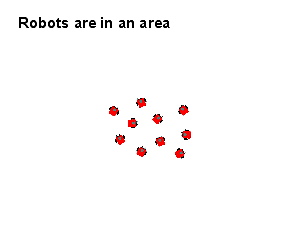
\includegraphics[width=\linewidth]{../ui_experiment/slide_images/Swarm_Robot_Control_-_Unknown_Number_of_Robots_0001.png}
	\end{subfigure}
	\begin{subfigure}{0.3\textwidth}
		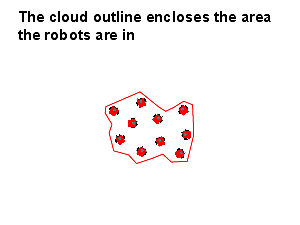
\includegraphics[width=\linewidth]{../ui_experiment/slide_images/Swarm_Robot_Control_-_Unknown_Number_of_Robots_0002.png}
	\end{subfigure}
	\begin{subfigure}{0.3\textwidth}
		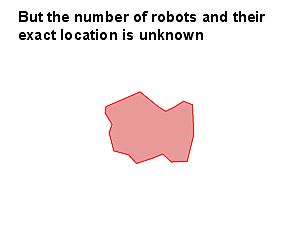
\includegraphics[width=\linewidth]{../ui_experiment/slide_images/Swarm_Robot_Control_-_Unknown_Number_of_Robots_0003.png}
	\end{subfigure}
	\caption{Instructional slides for the unknown number of robots condition, showing cloud representation of robot swarm.}
	\label{instructional_slides}
\end{figure}

\subsubsection{Selection Strategy}

At the end of the experiment, users were shown an image of a robot swarm, with a dotted line around it depicting a finger drag path around some of the robots. 
The users were told that the intent of this gesture was to select robots, and asked to indicate which robots in the image were selected, or in the unknown number of robots case, whether the gesture selected all of the robots or left any out. 
Users in the single robot case were shown the selection image with ten robots in it, because the with one robot, there are not enough robots to have a selection which may exclude some robots and include others. 

\begin{figure}
	\centering
	\begin{subfigure}{0.48\textwidth}
		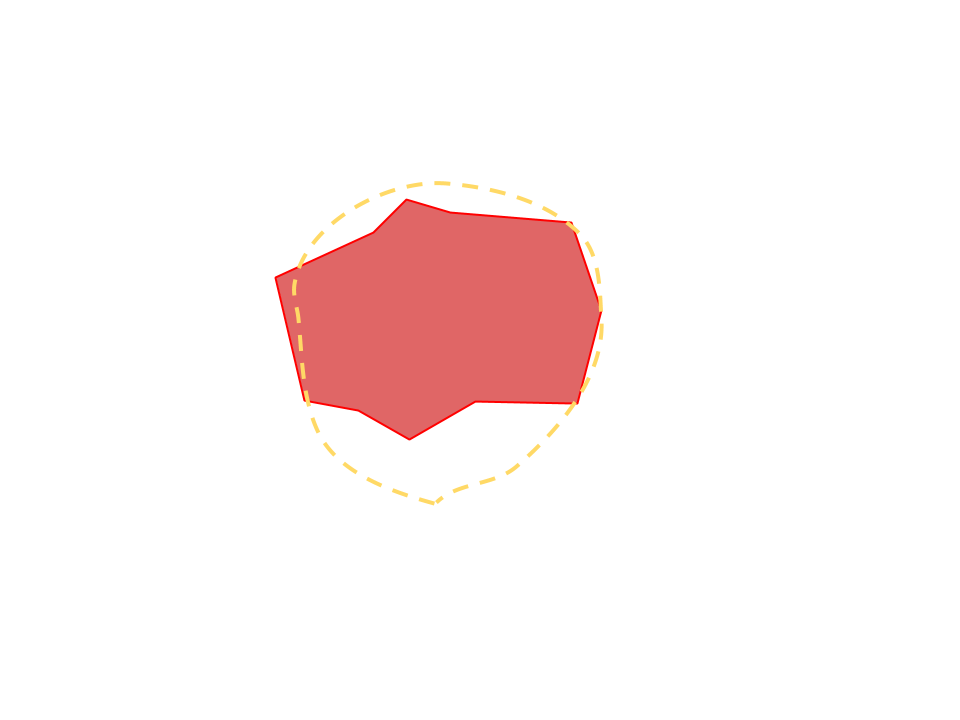
\includegraphics[width=\linewidth]{../Selection_Fuzz_X.png}
	\end{subfigure}
	\begin{subfigure}{0.48\textwidth}
		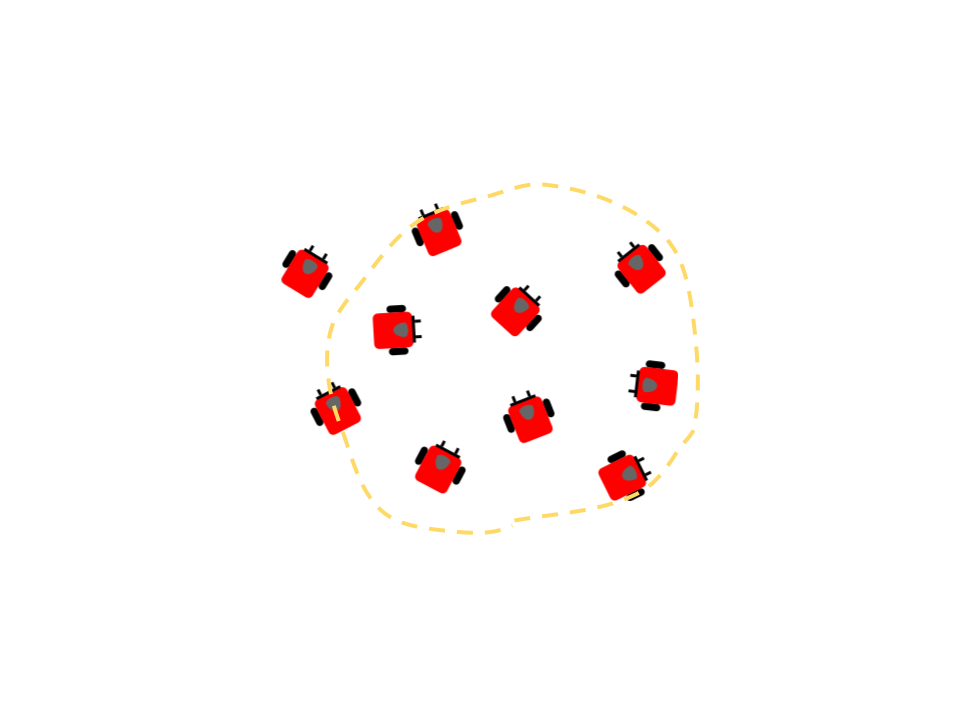
\includegraphics[width=\linewidth]{../Selection_Fuzz_10.png}
	\end{subfigure}
	\begin{subfigure}{0.48\textwidth}
		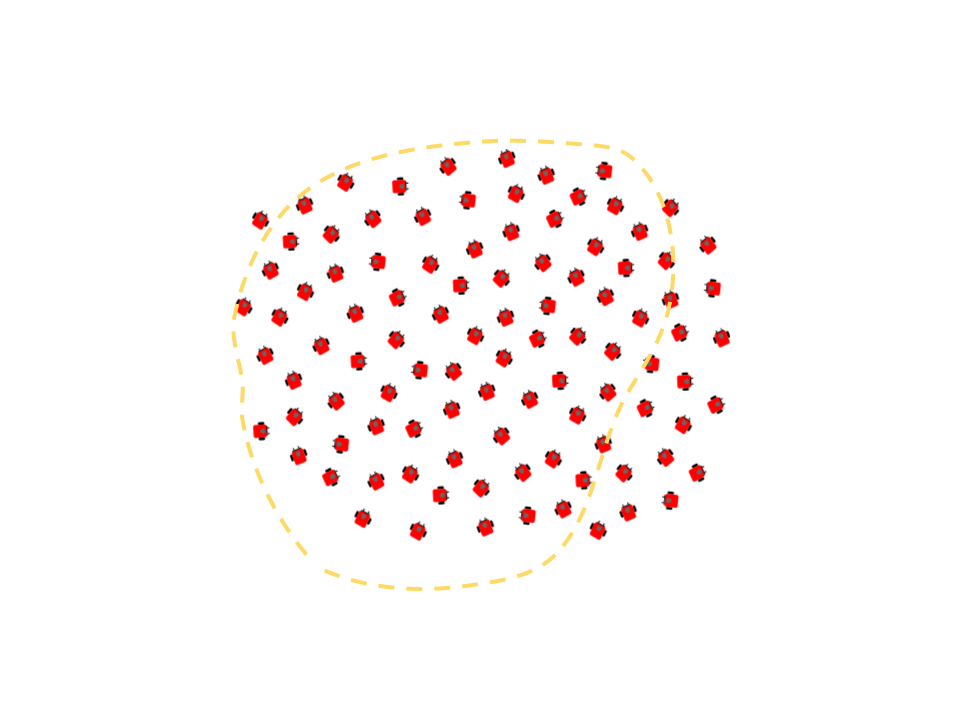
\includegraphics[width=\linewidth]{../Selection_Fuzz_100.png}
	\end{subfigure}
 	\begin{subfigure}{0.48\textwidth}
		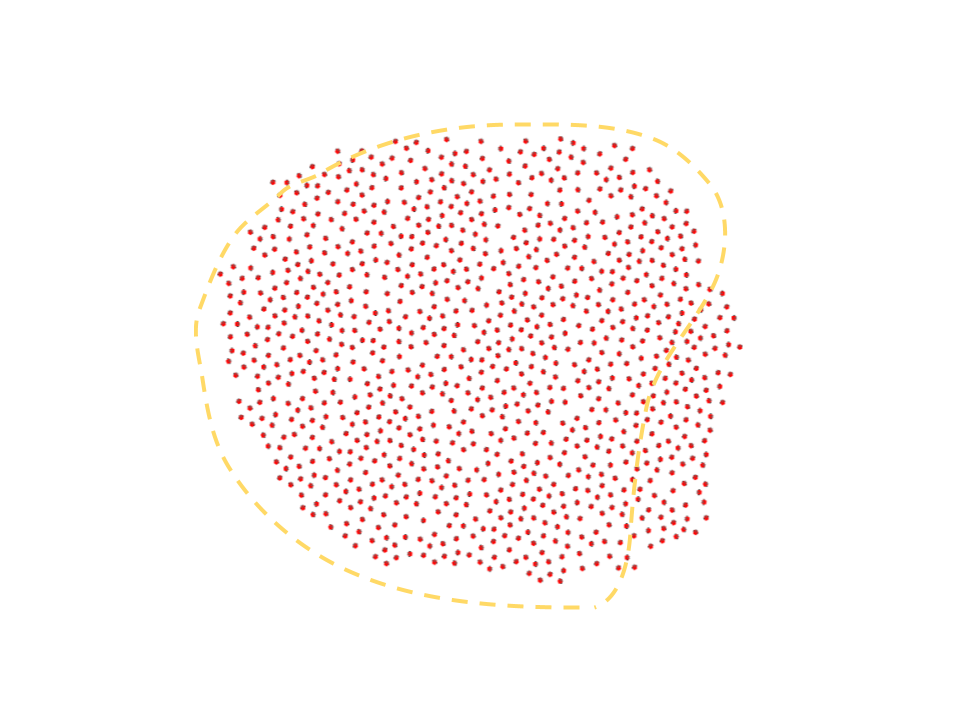
\includegraphics[width=\linewidth]{../Selection_Fuzz_1000.png}
	\end{subfigure}
		\caption{Images for selection strategy question.}
	\label{strategy_question}
\end{figure}

In the unknown number of robots case, 7 participants indicated that all the robots were selected, 3 of the participants indicated that some robots were left out, and one participant indicated that whether the selection included all of the robots could depend on the task. 

Because the 1 and 10 robot cases saw the same selection image, they are reported together. 
12 participants indicated that robots that were inside the selection or touched by the selection line should be considered selected. 
2 participants indicated that robots depicted with half or more of the robot inside the circle should be considered selected. 
One participant indicated that the robot half out of the circle should \emph{not} be selected. 
One participant indicated that robots on the border should be included or not included in the selection, depending on the task. \todo{Three answers are missing, find those and fix}
One user indicated that only the first robot touched should be selected, which is consistent with control strategies that move each robot individually. 

For the hundred robot case, 3 participants indicated that robots inside or touching the line were selected. 
3 participants said that robots should be mostly inside the line to be counted, with one participant stating that robots should be 80\% or more inside the line to count. 
2 participants indicated that robots should be more than halfway inside the line to be selected. 
One participant stated that only robots completely inside the line should be counted. \todo{One answer missing, find and fix}
 
In the thousand robot case, 7 participants indicated that robots inside or touching the line should be selected. 
2 participants indicated that robots must be completely inside the line to be selected. 
1 participant indicated that robots mostly inside the line should be selected. 

Overall, participants generally err on the side of inclusion, rather than exclusion of robots from selection.
If a user interface is required to include or exclude ambiguous elements from a selection, it appears that including ambiguous elements will satisfy users. 
User comments also suggested that ways to amend selections before further commanding the robots would be desirable.

 \begin{tabular}{ l l l l l}
   Condition & Completely inside & Half or more in & Touching line & Other\\
   \hline
   10 & 0 & 2 & 12 & 3 \\
   
   100 & 1 & 5 & 3 & 0 \\
   1000 & 2 & 1 & 7 & 0\\
   \hline
   Totals & 3 & 8 & 22 & 2 \\
 \end{tabular}

%It is interesting to note that two participants, one from the unknown number of robots case, and one from the 10 robot case, said that in cases of ambiguous selection, the system should add or remove robots from the selection based on the task. 
%As the system cannot predict the task it is about to be commanded to perform, it is likely best to err on the side of selecting too many robots, rather than too few. 



\subsubsection{Participant Demographics}

The experiment had 50 participants, 10 in each condition. 28 of the participants were male, 22 were female. The average age of participants was 22.1 years, with a standard deviation of 3.16. 

These demographics are representative of the location that the study was performed, the campus of an American college. 
It has been suggested that research in psychology focuses too much on a population that is WEIRD (Western, Educated, Industrialized, Rich, and Democratic), and that the results of such studies may not generalize beyond that population \citep{arnett2008neglected}.
However, for the purposes of this study, particularly assessing the influence of smartphone use on expectations of user interface gestures, it is useful to have a population with significant experience using smartphones, which are a product of both rich and industrialized societies. 
It is not proposed that the results of this work generalize to humanity as a whole.  

\subsection{Conclusions}

In future, it would be interesting to repeat this work with a condition that does not display the robots in the user interface at all. 
We expect that for conditions such as the ``move the crate'' tasks, the user would simply indicate the crate should move to area A, without concern for which robots perform the moving. 
However, such an interface would not afford indicating particular robots or groups, so tasks such as dividing the robots around an obstacle may become impossible to perform.

During this experiment, there were some cases where the users expectations of what was possible in the interface indicated a sort of ``metaphor failure" in the user interface. 
Natural User Interfaces, of which multitouch screens are an example, are supposed to be able to leverage users' understanding of the physical world, and how objects behave in it, to build affordances for objects on the screen. 
For example, a volume knob can be displayed as an actual knob, and the screen can react appropriately to attempts to rotate the knob. 
However, people know that the objects on the screen are not e.g. knobs, switches, and so on, but pictures of those things, drawn by the computer. 
As a result, the affordances are mixed. 
The knob may afford turning, but it also affords dragging around the screen or deletion, which a knob on a real radio does not afford. 
In this study, users were tasked with stopping the robots, which had begun to move around a wall to a target area. 
One user dragged the wall in front of the robots, and another user asked if they could move the wall. 
The wall was intended to represent an actual wall, which doesn't afford moving in the physical world, but it was represented in the experiment as a thick black line. 
It may be that the users would have not attempted to move the wall if it was more clearly represented as e.g. a stone or brick wall, and so had connotations of excessive weight. 
On the other hand, the users may have regarded it as what it actually was, an image of a wall on a computer screen, and decided that since images can be moved around the screen, the wall image can too. 
Attempting to experimentally determine if the representation affects how the user interacts with the wall may require a large number of users, as out of 50 participants, only 2 even mentioned the idea of moving the wall. 

In this experiment, some users were initially confused by the interface not responding. 
It may be that running this experiment on a computer, rather than a paper prototype, contributed to the user expectation that the system could react. 
Most users' experience with touch screens is that when they touch them, something visible happens nearly immediately. 
A system that does not visibly react, as in this experiment, is usually assumed to be broken, or waiting for further input, but no one expects printed documents to react to touch.
For future work, it may be desirable to structure attempts to elicit user gestures as in Wobbrock \emph{et al.}. 
The experiment described in this section showed the initial situation, and asked the users how they would make a specific change. 
Wobbrock \emph{et al.} showed the change occurring, and then asked the users what command they would issue to cause that result. 
Showing the response before asking for the gesture removes the expectation that the system will react. 

